\subsubsection{01.12.14}

\begin{enumerate}
	\item The time of beginning and ending of the meeting:
	15:30 - 19:00
	\item Purposes of the meeting:
	\begin{enumerate}
		\item To move the STB to the top of the last slat.
		
		\item To install П-shaped rigidity rib.
		
		\item To start elaborating the concept of the new bucket.
		
	\end{enumerate}
	\item Work that has been done:
	\begin{enumerate}
		\item MOB was moved to the top of the last slat.
		
		\begin{figure}[H]
			\begin{minipage}[h]{0.2\linewidth}
				\center  
			\end{minipage}
			\begin{minipage}[h]{0.6\linewidth}
				\center{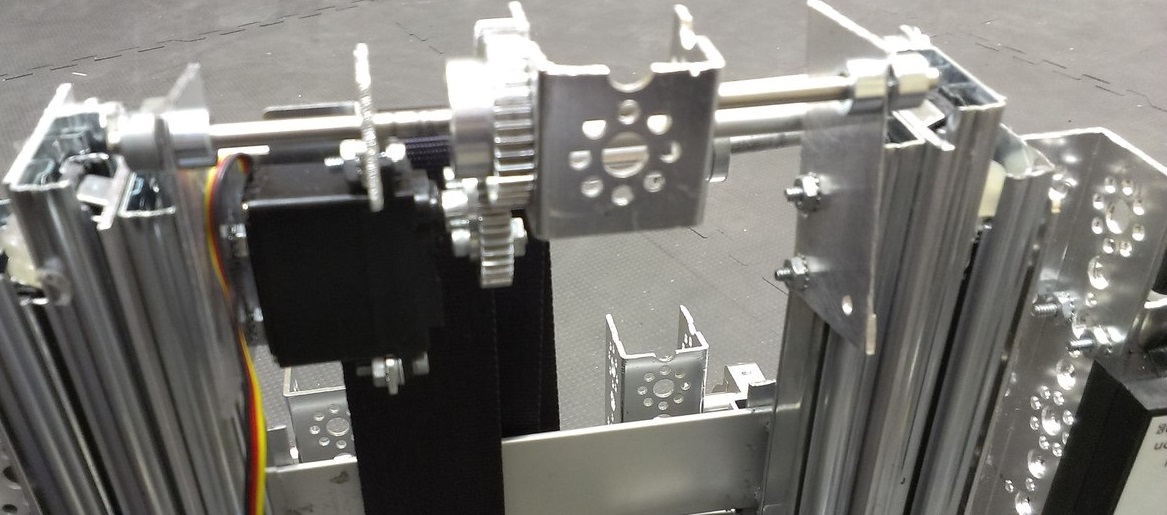
\includegraphics[scale=0.2]{days/01.12.14/images/01}}
				\caption{MOB}
			\end{minipage}
		\end{figure}
		
		\item П-shaped rigidity rib wasn't installed.
		
		\item It was decided to create the bucket so that on the bottom of the bucket there is pallet 7cm in height. A ramp is fixed on a front part of it. Then there is the part that opens on the front. It is needed for getting balls into the bucket. Then the bucket starts to narrow and at the top there is the hole slightly bigger than the big ball. The uniform narrowing doesn't allow the balls to get stuck inside the tube. After the bucket, there is a gutter that is fixed on the top pair of slats so that balls fall from the overturned bucket into the goal. The gutter ends by a folding element that directs balls to fall vertically - this increases the accuracy.
		
		\begin{figure}[H]
			\begin{minipage}[h]{0.2\linewidth}
				\center  
			\end{minipage}
			\begin{minipage}[h]{0.6\linewidth}
				\center{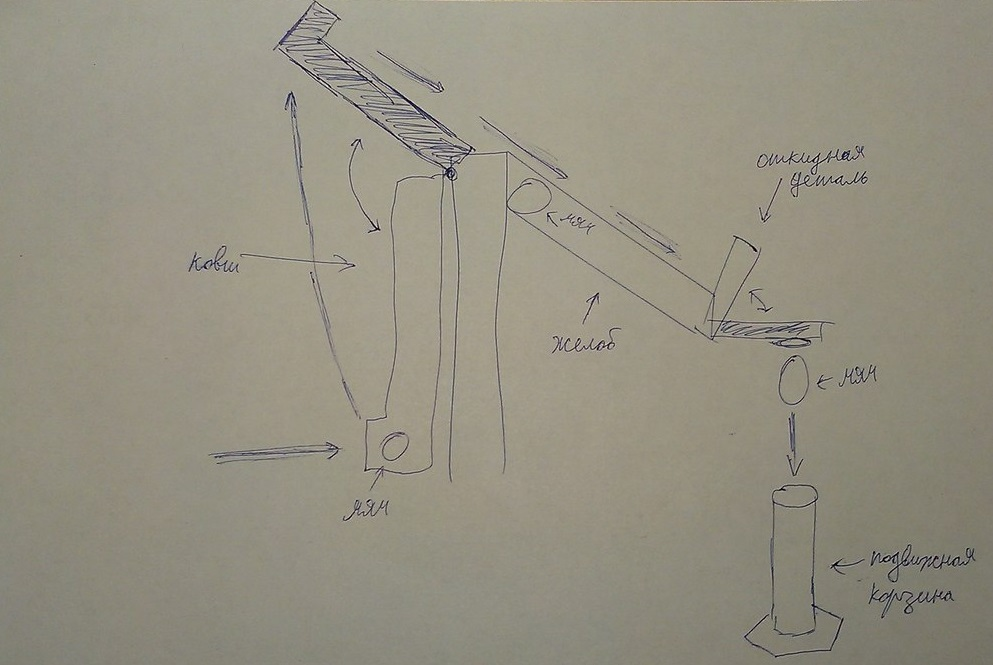
\includegraphics[scale=0.2]{days/01.12.14/images/02}}
				\caption{Concept of the bucket}
			\end{minipage}
		\end{figure}
		
	\end{enumerate}
	
	\item Results: 
	\begin{enumerate}
		\item MOB was moved to the top of the last slat.
		
		\item Rib of rigidity wasn't installed.
		
		\item Concept of the bucket elaborated
		
	\end{enumerate}
	
	\item Tasks for the next meetings:
	\begin{enumerate}
		\item To install П-shaped rib of rigidity.
		
		\item To start implementation of the bucket.
		
	\end{enumerate}     
\end{enumerate}
\fillpage